\section{Results}
%\subsection{Preliminary Results}
We piloted Monster Munch (N=68) and found users' confidence assessing macronutrients increased after using the app. Strong player-avatar-identification (PAID) and increased utilization of the crowdsourced community board were related to users' enjoyment of the app. Interestingly, lower PAID predicted greater recall of nutrition information, independent of prior nutrition knowledge. Findings suggest PAID may be an important mechanism in learning and highlights how fun, lightweight tools can prompt reflection and recall.





%%%%%% from my MA study
Statistical Package for the Social Sciences (SPSS version 27) was used to analyze the data and alpha was set at 0.05. 
%The first step analyzed participants' demographic information. A chi-square test of independence was performed to compare the frequency in the age ranges in the two-sided inoculation (\textit{n} = 120) and subversive (\textit{n} = 105) conditions. The relation between these variables was not significant, $(\chi^2 (5) = 2.996, p = .701)$. A chi square test of independence was performed to see if there were any significant relationships within gender, education level, income level, or prior game experiences between the two treatment groups. No statistical significance was found between the two groups in their gender $(\chi^2 (2) = 1.222, p = .543)$, education level $(\chi^2 (3) = 3.267, p = .352)$, income level $(\chi^2 (4) = 5.235, p = .264)$, and prior game experience $(\chi^2 (4) = 4.702, p = .319)$ as shown in Table~\ref{tab:learning}.''

%%%%%%%%%%%%%%%%
%%%%%%%%% comment out below for first draft

% This will be the github URL that we will share in the paper for the final draft. Not for anonymized version: \url{https://github.com/mlhwang/m4m} --- for preparing
% high-quality tables.

%%%%%%%%%%%%%%%%%%%%%%%%%%%%%%%

\subsection{confidence assessing macronutrients}

\begin{table}
  \caption{Frequency of Special Characters}
  \label{tab:freq}
  \begin{tabular}{ccl}
    \toprule
    Non-English or Math&Frequency&Comments\\
    \midrule
    \O & 1 in 1,000& For Swedish names\\
    % $\pi$ & 1 in 5& Common in math\\
    % \$ & 4 in 5 & Used in business\\
    % $\Psi^2_1$ & 1 in 40,000& Unexplained usage\\
  \bottomrule
\end{tabular}
\end{table}


\begin{table*}[t]
  \caption{The pre- and post-task means paired samples \textit{t}-test of identifying macronutrients (i.e., fat, carbohydrates, fiber) from meal photographs. \textsuperscript{***}$p<.01$, 
  \textsuperscript{**}$p<.05$, 
  \textsuperscript{*}$p<.1$}
  \label{tab:learning}
  \begin{tabular}{ c  l  r  c  r  c }
    \toprule
    Pair&N&Mean&Std. Dev&t&Sig. (2-sided)
    % \multicolumn{1}{|c|}{\textbf{Pair}}
    % & \multicolumn{1}{|c|}{\textbf {N}} 
    % & \multicolumn{1}{|c|}{\textbf {Mean}} 
    % & \multicolumn{1}{|c|}{\textbf {Std. Dev.}} 
    % & \multicolumn{1}{|c|}{\textbf {t}}
    % & \multicolumn{1}{|c|}{\textbf {Sig. (2-sided)}}\\
    \midrule                                  
    Confidence Pre to Post  &67 &-6.075  &14.274 &-3.484   &0.001**\\
    \bottomrule
\addlinespace[1ex]
\end{tabular}
  \vspace*{-\baselineskip}
\end{table*}




\subsection{nutritional learning }

\subsection{player avatar identification and community board}


SAMPLE OF REPORTING INDEPENDENT T-TESTS


``There was a statistically significant difference between pre- and post-gameplay PDQ means in Session 1 (\textit{M} = .386, \textit{SD} = 1.24, \textit{t}(56) = 2.36, \textit{p} = .022) but not in Session 2 in the subversive group.'' \textcolor{orange}{Remember in this example reporting EFFECT SIZE is not included. We must report that.}



SAMPLE TABLE TO summarize numeric data and indicate p values. \textcolor{orange}{Maybe it does look better to create the Tables without borderlines on the sides so they look more open?}




\textcolor{orange}{Take from \cite{cuthbert2019effects}:THIS SHOULD BE A GOOD MODEL FOR REPORTING ANOVAs if we use those stats techniques.   $\eta_{\text{p}}^{2}= some number to report partial eta square$.}


To set a wider table, which takes up the whole width of the page's
live area, use the environment \textbf{table*} to 
desirable. Immediately following this sentence is the point at which
Table~\ref{tab:commands} is included in the input file; again, 

\begin{table*}
  \caption{Some Typical Commands}
  \label{tab:commands}
  \begin{tabular}{ccl}
    \toprule
    Command &A Number & Comments\\
    \midrule
    \texttt{{\char'134}author} & 100& Author \\
    \texttt{{\char'134}table}& 300 & For tables\\
    \texttt{{\char'134}table*}& 400& For wider tables\\
    \bottomrule
  \end{tabular}
\end{table*}

Always use midrule to separate table header rows from data rows, and
use it only for this purpose. 



\subsection{Figures}

The ``\verb|figure|'' environment should be used for figures.
\begin{figure}[h]
  \centering
  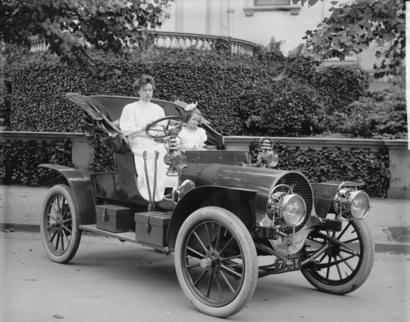
\includegraphics[width=\linewidth]{template_files/sample-franklin}
  \caption{1907 Franklin Model D roadster. Photograph by Harris \&
    Ewing, Inc. [Public domain], via Wikimedia
    Commons. (\url{https://goo.gl/VLCRBB}).}
  \Description{A woman and a girl in white dresses sit in an open car.}
\end{figure}

Your figures should contain a caption which describes the figure to
the reader.

Figure captions are placed {\itshape below} the figure.



A figure description must be unformatted plain text less than 2000
characters long (including spaces).  {\bfseries Figure descriptions
  should not repeat the figure caption – their purpose is to capture
  important information that is not already provided in the caption or
  the main text of the paper.} 

\subsection{The ``Teaser Figure''}

A ``teaser figure'' is an image, or set of images in one figure, that
are placed after all author and affiliation information, and before
the body of the article, spanning the page. If you wish to have such a
figure in your article, place the command immediately before the
\verb|\maketitle| command:
\begin{verbatim}
  \begin{teaserfigure}
    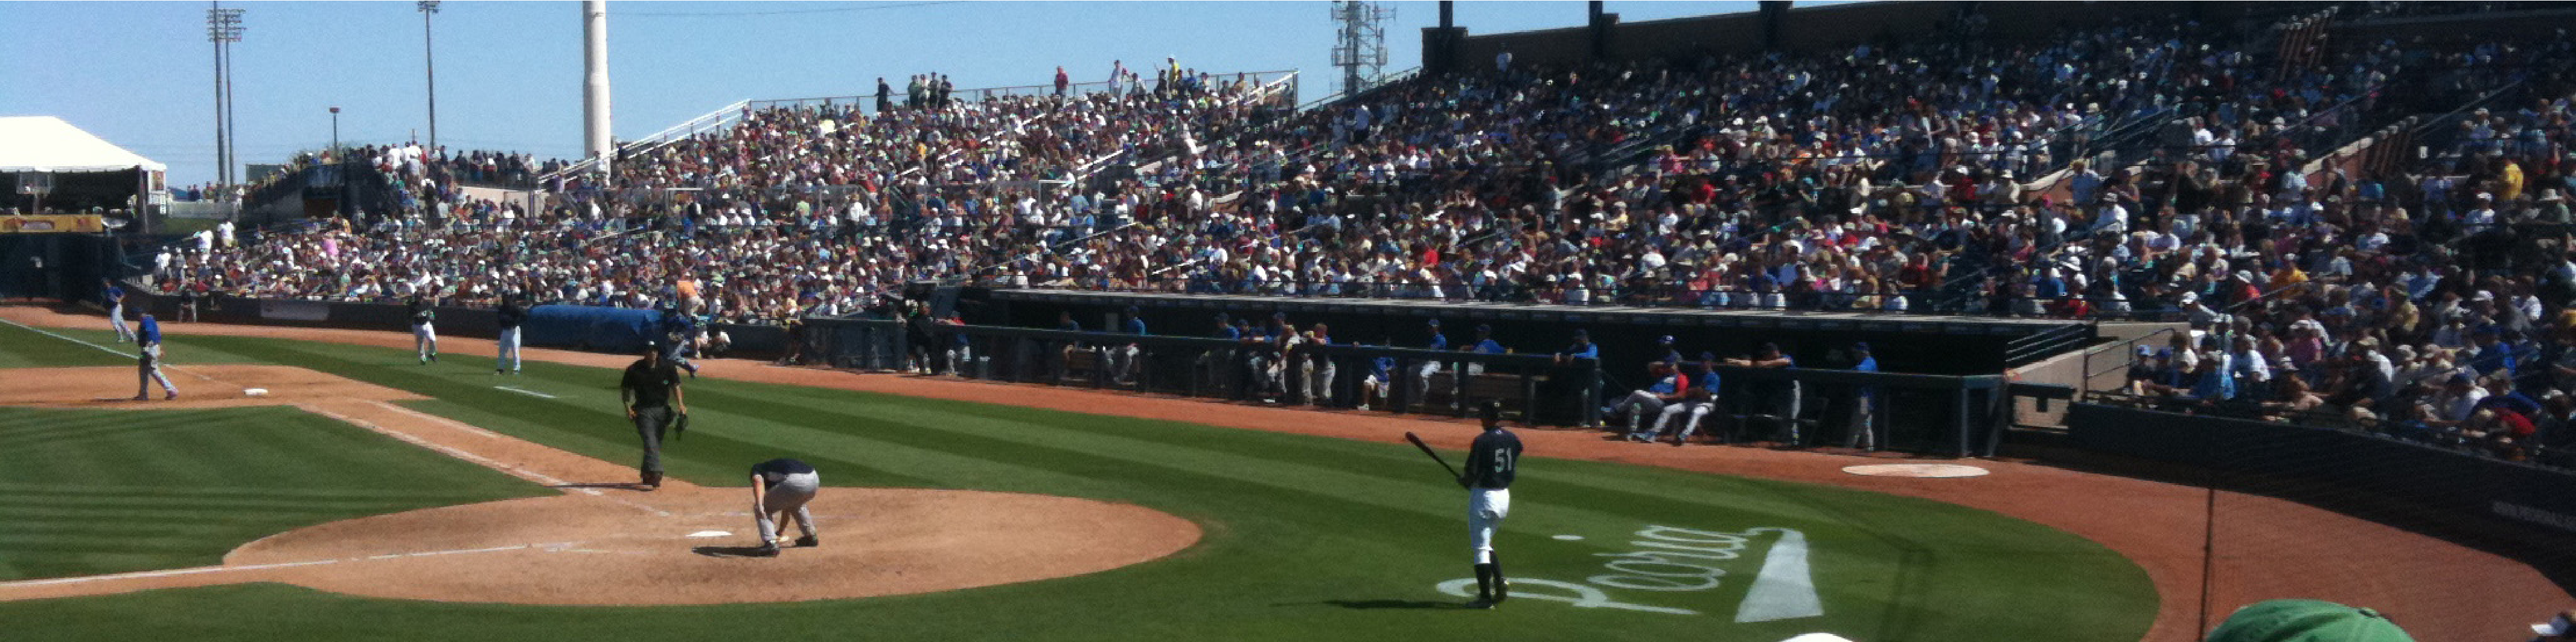
\includegraphics[width=\textwidth]{samples/template_files/sampleteaser}
    \caption{figure caption}
    \Description{figure description}
  \end{teaserfigure}
\end{verbatim}